\documentclass{beamer}
\usetheme{Madrid}

\usepackage{geometry}
\usepackage{scrextend}
\usepackage[absolute, overlay]{textpos}
\usepackage[utf8]{inputenc}
\usepackage{svg}
\usepackage{adjustbox}
\usepackage{graphicx}
\usepackage{xcolor}
\usepackage{transparent}
\usepackage{caption}
% \usepackage{tocloft}

%Information to be included in the title page:
\title[Seminario 8]{\textbf{Impossibilità del consenso nel modello a rete asincrono: una soluzione randomizzata}}
\subtitle{\scriptsize \textit{Seminario 8}}
\author[Liberatore, Mulone, Palazzo, Porta]{Daniele Liberatore, Alberto Mulone, \\ Matteo Palazzo, Stefano Porta}
\institute[]{Università degli Studi di Torino}
\date{20 gennaio 2021}

\hypersetup{
  pdfauthor={Daniele Liberatore, Alberto Mulone, Matteo Palazzo, Stefano Porta},
  pdftitle={Impossibilità del consenso nel modello a rete asincrono: una soluzione randomizzata},
  pdfproducer={LaTeX with hyperref},
  pdfcreator={latexmk}
}

\iffalse
\AtBeginSection[]{
  \begin{frame}
  \vfill
  \centering
  \begin{beamercolorbox}[sep=8pt,center,shadow=true,rounded=true]{title}
    \usebeamerfont{title}\insertsectionhead\par%
  \end{beamercolorbox}
  \vfill
  \end{frame}
}
\fi

\AtBeginSection[]
{
    \begin{frame}
        \frametitle{Overview}
        \tableofcontents[currentsection]
    \end{frame}
}

\begin{document}
{
    \beamertemplatenavigationsymbolsempty
    \setbeamertemplate{footline}{}
    \usebackgroundtemplate{
        \adjustbox{trim=-8cm 0 0 -4.5cm}{
            \transparent{0.3}\includesvg[scale=0.4,keepaspectratio=true]{unito-logo.svg}
        }
    }
    \begin{frame}
        \titlepage
    \end{frame}
    \addtocounter{framenumber}{-1}
}
% \frame{\titlepage}

    \iffalse
    \begin{frame}{Overview}
        \tableofcontents
    \end{frame}
    \fi

% Capitolo 17

    \section{Introduzione}
    \begin{frame}{Modello a rete asincrono}
        \begin{textblock*}{\textwidth}
            (0mm, 12mm)
            \begin{itemize}
                \item Un modello a rete di tipo \textit{send/receive} è costituito da processi interconnessi tramite appositi canali.
                \item Per canale si intende una coda FIFO \textit{affidabile} (i.e. i messaggi ivi contenuti sono ordinati e non duplicati).
                \item Un processo invia un messaggio tramite l'apposita azione di output \texttt{send}, mentre la lettura avviene tramite l'azione di input \texttt{receive}.
                \item Quando un singolo messaggio può essere inviato a molteplici destinatari si parla di modello a rete \textit{broadcast}.
            \end{itemize}
        \end{textblock*} 

        \begin{textblock*}{0.45\textwidth}
            (8mm, 60mm)
            \begin{block}{}
                \begin{figure}
                    \centering
                    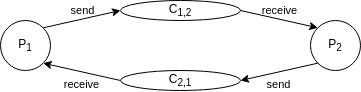
\includegraphics[scale=0.4]{modello_a_rete.png}
                \end{figure}
            \end{block}
        \end{textblock*}
        \begin{textblock*}{0.3\textwidth}
            (75mm, 52.5mm)
            \begin{block}{}
                \begin{figure}
                    \centering
                    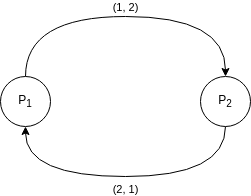
\includegraphics[scale=0.4]{modello_a_rete_digrafo.png}
                \end{figure}
            \end{block}
        \end{textblock*}
    \end{frame}

    \begin{frame}{Fault-tolerance}
        Un processo può fallire semplicemente stoppandosi in qualsiasi momento della sua esecuzione. Definiamo questo tipo di fallimento \textbf{stopping failure}.
        \\[10pt]
        Un fallimento di questo tipo può essere modellato aggiungendo a ogni processo $P_{i}$ un evento di input chiamato \textit{$stop_{i}$}, questo causa il fallimento del processo cambiandone lo stato e disabilitando tutti i suoi task.
        \\[10pt]
        Un sistema A interfacciato verso gli utenti U è fault-tolerant rispetto a \textit{f} fallimenti se rispetta la seguente condizione di liveness:
        \begin{block}{f-failure termination}
            Per ogni esecuzione del sistema composto $A \times U$ in cui occorrono degli eventi di stop su al più \textit{f} porte, ogni invocazione su una porta non-fallita ha una risposta.
        \end{block}

    \end{frame}

    \section{Da modello a rete al modello a memoria condivisa}
    \begin{frame}{Da modello a rete al modello a memoria condivisa}
        \begin{block}{Perché convertire un modello a rete in uno a memoria condivisa?}
            \begin{itemize}
                \item I sistemi a memoria condivisa sono di più facile comprensione e offrono una maggiore espressività.
                \item Esistono numerosi algoritmi già sviluppati per i modelli a memoria condivisa.
                \item Il modello a rete simula ed eredita le caratteristiche proprie di un sistema a memoria condivisa.
            \end{itemize}
        \end{block}
    \end{frame}

    \begin{frame}{I-simulazione}
        Un sistema B \textbf{simula} un sistema A se il suo comportamento è indistinguibile per un insieme di utenti esterni U.

        \begin{block}{I-simulazione}
            Un sistema B composto da n processi $P_{i}$ con $1 \leq i \leq n$, è una I-simulazione (dove I indica un determinato insieme di porte) di A se per ogni esecuzione $\alpha$ di B e per ogni collezione di utenti $U_{i}$, esiste una esecuzione $\alpha'$ di A con gli stessi utenti per cui:
            \begin{itemize}
                \item $\alpha$ e $\alpha'$ sono indistinguibili agli utenti U. % spiegare a voce cosa signigica indistinguibili
                \item per ogni \textit{i} un evento $stop_{i}$ occorre in $\alpha$ se e solo se occorre in $\alpha'$
            \end{itemize}
        \end{block}

    \end{frame}

    \subsection{Equivalenza tra modello a rete e a memoria condivisa}
    \begin{frame}{SimpleSRSim - 1}
        \begin{textblock*}{\textwidth}
            (0mm, 12mm)
            \begin{itemize}
                \item Supponiamo di voler creare un sistema asincrono a memoria condivisa $B$ che ne simuli uno a rete $A$.
                \item Per ogni arco di $A$ che collega due processi $P_i$ e $P_j$, nel sistema B si crea una variabile condivisa $x(i, j)$ modificabile solamente da $P_i$ e leggibile esclusivamente da $P_j$.%\footnote{Si tratta di una variabile condivisa single-reader/single-writer}
                \item Ogni variabile condivisa del tipo $x(i,j)$ contiene una propria coda di messaggi, utile per l’emulazione delle operazioni di base di un sistema a rete.
            \end{itemize}
        \end{textblock*}
        \begin{textblock*}{0.65\textwidth}
            (45mm, 50mm)
            \begin{block}{Variabile condivisa single-reader/single-writer}
                \begin{figure}
                    \centering
                    % Freccia tratteggiata: operazione di lettura
                    % Freccia non tratteggiata: operazione di scrittura
                    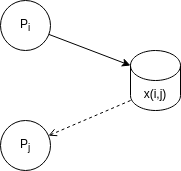
\includegraphics[scale=0.4]{struttura_di_base.png}
                \end{figure}
            \end{block}
        \end{textblock*}
    \end{frame}

    \begin{frame}{SimpleSRSim - 2}
        \begin{textblock*}{\textwidth}
            (0mm, 12mm)
            \begin{itemize}
                \item L'invio del messaggio $m$ dal processo $i$ al processo $j$ viene emulato aggiungendo il messaggio $m$ al fondo della coda contenuta in $x(i, j)$.
                \item Un generico processo $i$ verifica ciclicamente la presenza di eventuali nuovi messaggi ricevuti da un qualche processo $j$ esaminando il contenuto della variabile $x(j, i)$.
                \item L'elaborazione di un generico messaggio $m$ rimane invariata.
            \end{itemize}
        \end{textblock*}
        \begin{textblock*}{0.4\textwidth}
            (8mm, 45mm)
            \begin{block}{Modello a rete}
                \begin{figure}
                    \centering
                    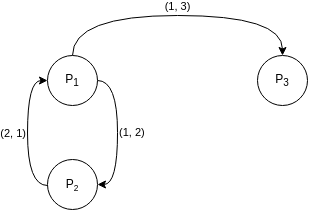
\includegraphics[scale=0.4]{test_sr.png}
                \end{figure}
            \end{block}
        \end{textblock*}
        \begin{textblock*}{0.45\textwidth}
            (65mm, 45mm)

            \begin{block}{Modello a memoria condivisa}
                \begin{figure}
                    \centering
                    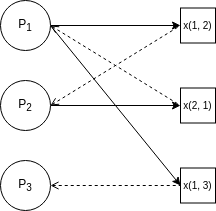
\includegraphics[scale=0.4]{test_sm.png}
                \end{figure}
            \end{block}
        \end{textblock*}
    \end{frame}

    \begin{frame}{SimpleBCastSim - 1}
        \begin{itemize}[<+->]
            \item In questo caso, per ogni $P_{i}$ con $1 \leq i \leq n$, il sistema \textit{B} ha una variabile condivisa $x(i)$ a singolo scrittore/multipli lettori.
            \newline La variabile è scrivibile da $P_{i}$ e leggibile da tutti i processi ($P_{i}$ incluso), e contiene una coda di messaggi, inizialmente vuota.
            \item Come con SimpleSRSim, un processo $P_{i}$ di \textit{B} simula direttamente lo stesso i-esimo processo di \textit{A}.
        \end{itemize}
    \end{frame}

    \begin{frame}{SimpleBCastSim - 2}
        \begin{block}{Broadcast}
            Per simulare un'azione $bcast(m)_{i}$ di $P_{i}$, il processo \textit{i} di \textit{A} aggiunge il messaggio \textit{m} alla fine della coda presente nella variabile \textit{x(i)}.
            \begin{figure}
                \centering
                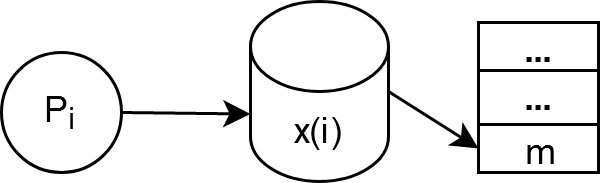
\includegraphics[scale=0.3]{Broadcast.png}
            \end{figure}
        \end{block}
    \end{frame}

    \begin{frame}{SimpleBCastSim - 3}
        \begin{block}{Ricezione}
            Il processo \textit{i} periodicamente controlla tutte le variabili \textit{x(j)} (inclusa \textit{x(i)}), per verificare se sono presenti dei nuovi messaggi. Se effettivamente ve ne sono, li gestisce allo stesso modo di $P_{i}$.
            \begin{figure}
                \centering
                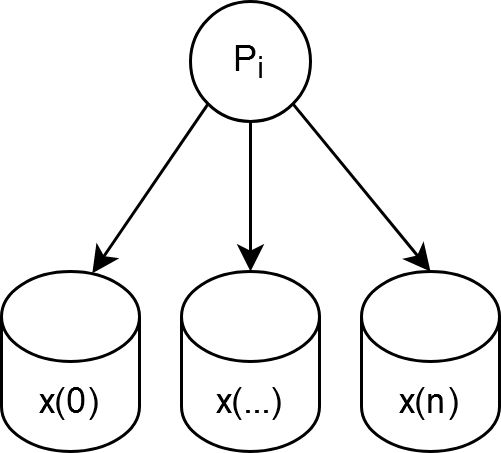
\includegraphics[scale=0.26]{BroadcastReceive.png}
            \end{figure}
        \end{block}
    \end{frame}

% SimpSRSim
% SimpBCastSim

    \begin{frame}{Equivalenza tra modello Send/Receive e Broadcast}
        \begin{block}{Teorema}
            Dato un generico sistema asincrono a rete broadcast A esiste un sistema asincrono send / receive B che è una I-simulazione di A.
        \end{block}

        \vspace{0.5cm}

        Data questa equivalenza da ora in poi supporremo di lavorare in sistemi asincroni a rete broadcast, in quanto permettono la stesura di algoritmi più intuitivi e più facilmente dimostrabili.
    \end{frame}

    \begin{frame}{Problema del consenso}
        Un insieme di $n$ utenti $U_{i}$ interagiscono con un sistema di n processi $P_{i}$ attraverso un certo modello di comunicazione, ogni utente $U_{i}$ inizializza con un certo valore \textit{v} il processo $P_{i}$ attraverso l'azione $init(v)_{i}$.
        \\[10pt]
        I processi $P_{i}$ interagiranno tra di loro per compiere una scelta unanime di un certo valore $v$ da comunicare agli utenti $U_{i}$ attraverso l'azione $decide(v)_{i}$.

        %%%%%%%%%%%%%%% COMMENTO %%%%%%%%%%%%%%%%%%%%%
        \iffalse
        Ogni processo può essere soggetto a un \textbf{stopping failure}, ovvero può smettere di funzionare senza nessun avviso. Questo può essere modellato attraverso delle azioni di input chiamate $stop_{i}$ le quali non fanno altro che disabilitare ogni azione localmente controllata del processo $P_{i}$. Una esecuzione è detta failure-free se non contiene eventi di $stop$
        \fi
    \end{frame}

    \subsection{Il problema del consenso}

    \begin{frame}{Impossibilità del consenso nel modello a rete}

        Il modello a rete eredita dal modello a memoria condivisa l'impossibilità del consenso.

        \begin{block}{Teorema}
            Dato un qualsiasi sistema asincrono a rete composto da un numero $n \geq 2$ di processi, non esiste un algoritmo che risolva il problema del consenso e garantisca la \textit{1-failure termination}.
        \end{block}
    \end{frame}

    \begin{frame}{Dimostrazione}
        \begin{itemize}
            \item Supponiamo per \textbf{assurdo} che esista un algoritmo \texttt{A} in grado di risolvere il problema del consenso in un sistema asincrono a rete broadcast e che garantisca la 1-failure termination.
            \item Per quanto dimostrato è possibile ottenere un algoritmo B per un sistema a modello a memoria condivisa che è un n-simulazione di \texttt{A}.
            \item Pertanto \texttt{B} risolverebbe il problema del consenso garantendo la 1-failure termination. Questo però contraddice il teorema dell'impossibilità del consenso nel modello a memoria condivisa.
        \end{itemize}
    \end{frame}

% Capitolo 21


    \section{Una soluzione randomizzata}

    \begin{frame}{Una soluzione randomizzata}
        Poichè problema del consenso è di vitale importanze in diversi settori, come ad esempio la gestione di transazioni in database distribuiti; è stato necessario sviluppare degli espedienti:
        \vspace{0.2cm}
        \begin{itemize}
            \item Indebolimento dei requisiti di correttezza
            \item Rafforzamento del modello attraverso:
            \vspace{0.2cm}

            %%% ha senso ??? %%%
            \begin{itemize}
                \item \textbf{Utilizzo della randomizzazione}
                \item Failure detection
                \item Consenso su un insieme di valori
                \item Consenso parziale
            \end{itemize}
        \end{itemize}
    \end{frame}

    \begin{frame}{Requisiti di correttezza}
        Un sistema A risolve il problema del consenso se per ogni collezione di utenti U garantisce:
        \begin{itemize}
            \item \textbf{Well-formedness}: ogni interazione tra il sistema ed utenti $U_{i}$ è ben formata:
            \begin{itemize}
                \item Non contiene azioni ripetute di \textit{init},
                \item Non contiene azioni ripetute di \textit{decide},
                \item Ogni \textit{decide} è preceduto un \textit{init}.
            \end{itemize}
            \item \textbf{Agreement}: Tutti i valori di decisione sono uguali.
            \item \textbf{Validity}: Se tutte le azioni di \textit{init} danno in input lo stesso valore \textit{v}, allora l'unico valore che può essere deciso è \textit{v}.
            \item \textbf{Failure-free termination}: In ogni esecuzione failure-free in cui un \textit{init} è stata fatta su ciascuna porta, un evento \textit{decide} viene fatto su tutte le porte.
        \end{itemize}
    \end{frame}

    \begin{frame}{Requisiti di terminazione}
        Un sistema A composto da n processi $P_{i}$ è \textit{fault-tolerant}, rispetto a \textit{f} ($0 \leq f \leq n$) fallimenti, se soddisfa la seguente proprietà di terminazione:
        \begin{block}{f-failure termination}
            In ogni esecuzione fair in cui degli eventi di \textit{init} occorrono su tutte le porte, se ci sono al più \textit{f} eventi di \textit{stop}, allora un evento di \textit{decide} occorre su tutte le porte non-fallite.
        \end{block}
        % potremmo parlare di 1-failure termination e n-failure termination
    \end{frame}

    \subsection{Algoritmo di BenOr}
    \begin{frame}{Algoritmo di BenOr}
        \begin{itemize}
            \item L'algoritmo di BenOr funziona con $n > 3f$ processi e con l'insieme di valori di scelta $V = \{0, 1\}$.

            \item Ogni $P_{i}$ esegue una serie infinita di \textbf{stage} numerati in maniera incrementale e ognuna di essa è divisa in due \textbf{round}.

            \item I processi nei vari stage si scambiano messaggi i quali contengono:
            \begin{itemize}
                \item un tag che può essere o R (Report) o P (Propose);
                \item un numero che indica lo stage corrente, indicato con $s$;
                \item un valore definito nel round indicato con $v$.
            \end{itemize}

            \item L'algoritmo continua la propria esecuzione anche dopo aver effettuato una $decide(v)_i$.
        \end{itemize}
    \end{frame}

    \begin{frame}{Algoritmo di BenOr - Inizializzazione}
        \begin{itemize}
            \item Ogni processo $P_{i}$ ha due variabili locali $x$ e $y$ inizializzate a $null$.

            \item All'occorrenza di un input $init(v)_{i}$ sul processo $P_{i}$ viene assegnato ad $x$ il valore $v$ ($v \in V$).

            \item La numerazione degli stage inizia con il valore 0 e viene incrementato all'inizio di ogni round 1.
        \end{itemize}
    \end{frame}


    \begin{frame}{Algoritmo di BenOr - Round 1}
        \begin{itemize}
            \item $P_{i}$ invia in broadcast agli altri processi un messaggio della forma \mbox{(R, s, x)}.

            \item Successivamente attende di ricevere messaggi (R, s, *) da n - f processi\footnote{Il valore indicato da * può essere 0 o 1}.

            \item Se tutti i messaggi ricevuti hanno lo stesso valore $v$ allora salva nella variabile $y$ il valore $v$.

            \item altrimenti salva in $y$ il valore null.

        \end{itemize}
    \end{frame}


    \begin{frame}{Algoritmo di BenOr - Round 2}

        \begin{itemize}
            \item $P_{i}$ invia in broadcast agli altri processi un messaggio della forma \mbox{(P, s, y)}.

            \item Successivamente attende di ricevere messaggi (P, s, *) da n - f processi\footnote{Il valore indicato da * può essere 0, 1 o null}.

            \item Se tutti i messaggi ricevuti hanno lo stesso valore $v$ e $v$ diverso da null allora salva in $x$ il valore $v$ ed esegue l'azione $decide(v)_{i}$ (se non è già stato fatto in uno stage precedente).

            \item altrimenti Se almeno $n - 2f$ messaggi ricevuti hanno lo stesso valore $v$ e $v$ diverso da null allora salva in $x$ il valore $v$.

            \item altrimenti viene assegnato ad $x$ un valore scelto \underline{casualmente}\footnote{Quest'azione rende probabilistico l'intero algoritmo.} dall'insieme V.
        \end{itemize}
    \end{frame}

% dimostrazione benor 

% simulazione benor

\begin{frame}{Considerazioni}
    \begin{block}{Teorema}
        L'algoritmo di BenOr garantisce le proprietà di well-formdness, validity e agreement. Inoltre viene garantita con probabilità 1 che tutti i processi non-falliti prima o poi decidono.
    \end{block}
\end{frame}

\subsection{Simulazione}
\begin{frame}{Simulazione - Configurazione iniziale}
\begin{figure}
    \centering
    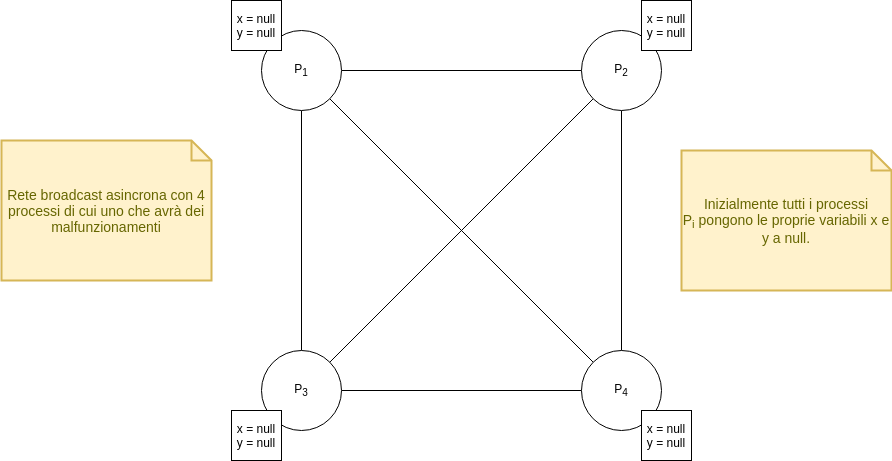
\includegraphics[scale=0.35]{simulazione/simulazione1.png}
\end{figure}
\end{frame}

\begin{frame}{Simulazione - Stage 0 (Inizializzazione)}
\begin{figure}
    \centering
    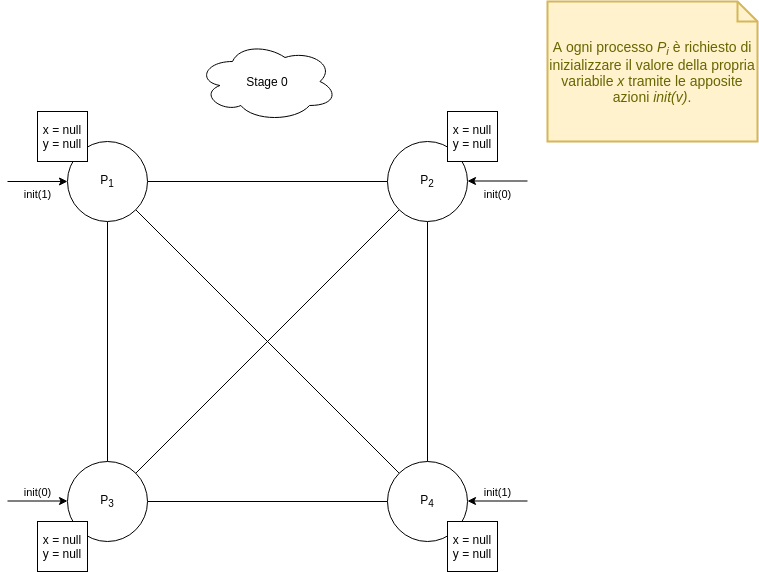
\includegraphics[scale=0.35]{simulazione/simulazione2.png}
\end{figure}
\end{frame}

\begin{frame}{Simulazione - Stage 1 (Report 1/2)}
\begin{figure}
    \centering
    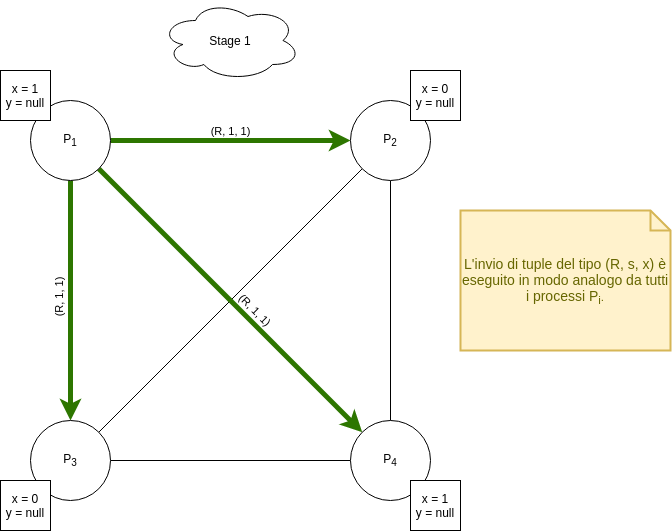
\includegraphics[scale=0.35]{simulazione/simulazione3.png}
\end{figure}
\end{frame}

\begin{frame}{Simulazione - Stage 1 (Report 2/2)}
\begin{figure}
    \centering
    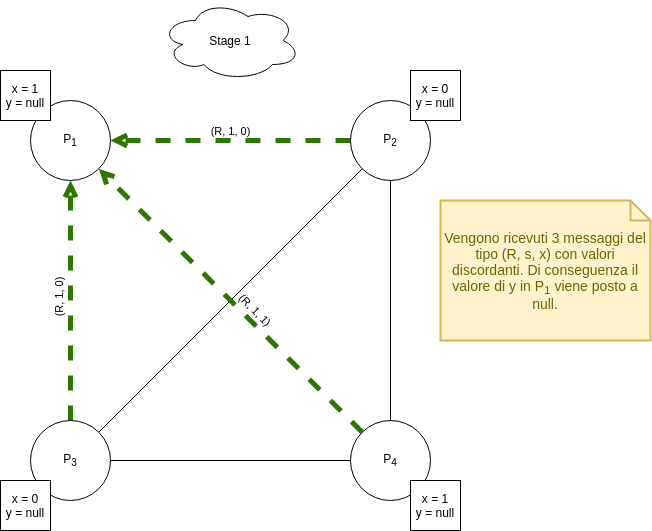
\includegraphics[scale=0.35]{simulazione/simulazione4.png}
\end{figure}
\end{frame}

\begin{frame}{Simulazione - Stage 1 (Propose 1/2)}
\begin{figure}
    \centering
    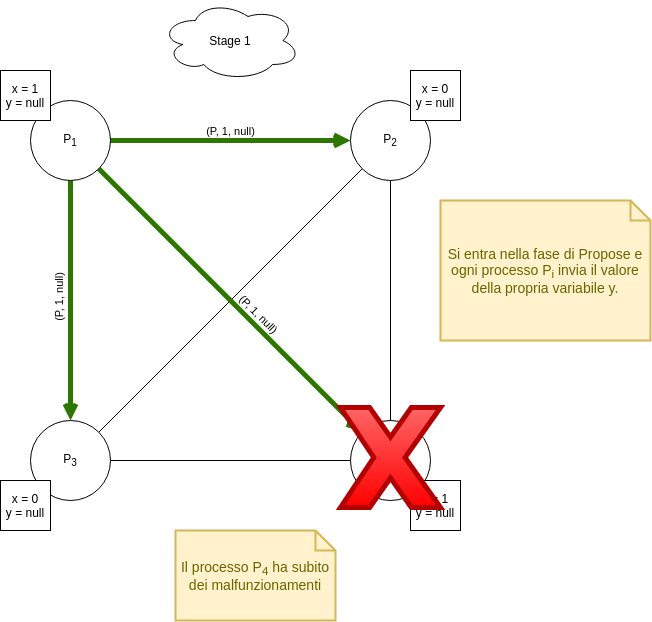
\includegraphics[scale=0.35]{simulazione/simulazione5.png}
\end{figure}
\end{frame}

\begin{frame}{Simulazione - Stage 1 (Propose 2/2)}
\begin{figure}
    \centering
    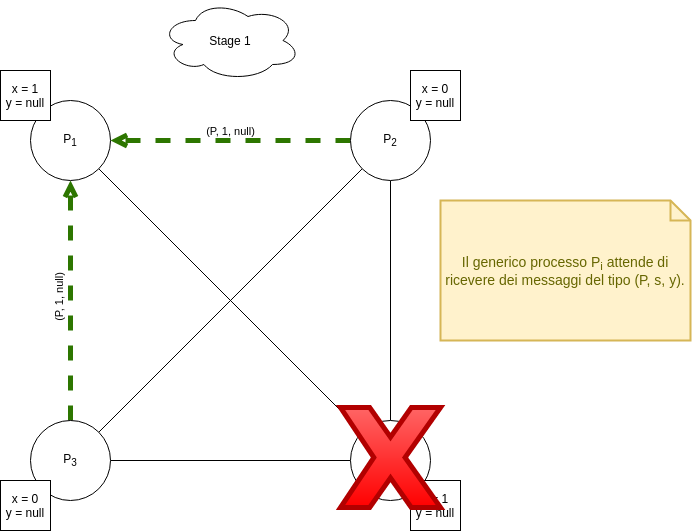
\includegraphics[scale=0.35]{simulazione/simulazione6.png}
\end{figure}
\end{frame}

\begin{frame}{Simulazione - Stage 1 (Scelta casuale)}
\begin{figure}
    \centering
    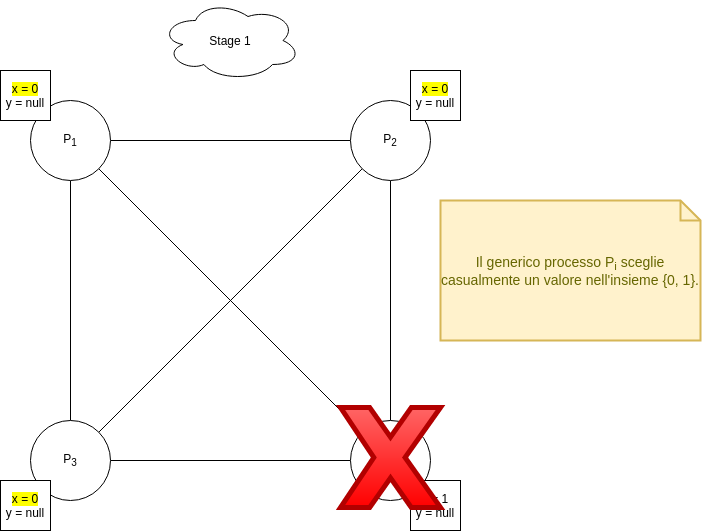
\includegraphics[scale=0.35]{simulazione/simulazione7.png}
\end{figure}
\end{frame}

\begin{frame}{Simulazione - Stage 2 (Report 1/2)}
\begin{figure}
    \centering
    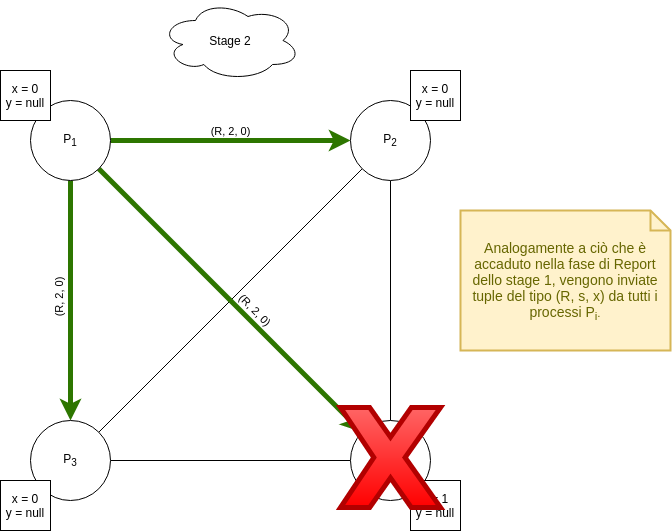
\includegraphics[scale=0.35]{simulazione/simulazione8.png}
\end{figure}
\end{frame}

\begin{frame}{Simulazione - Stage 2 (Report 2/2)}
\begin{figure}
    \centering
    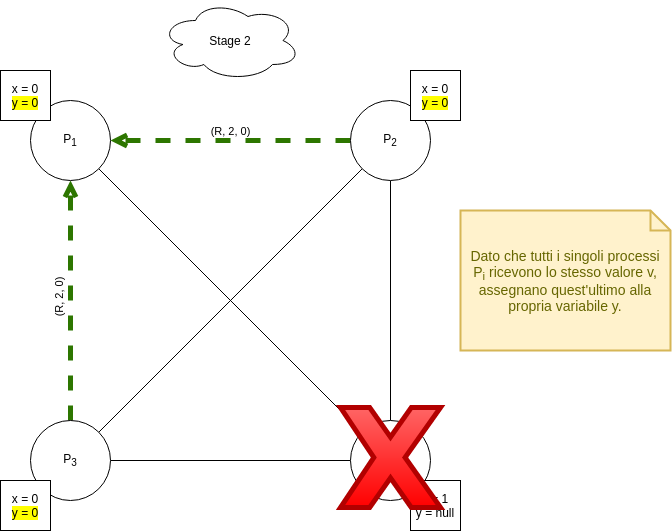
\includegraphics[scale=0.35]{simulazione/simulazione9.png}
\end{figure}
\end{frame}

\begin{frame}{Simulazione - Stage 2 (Propose 1/2)}
\begin{figure}
    \centering
    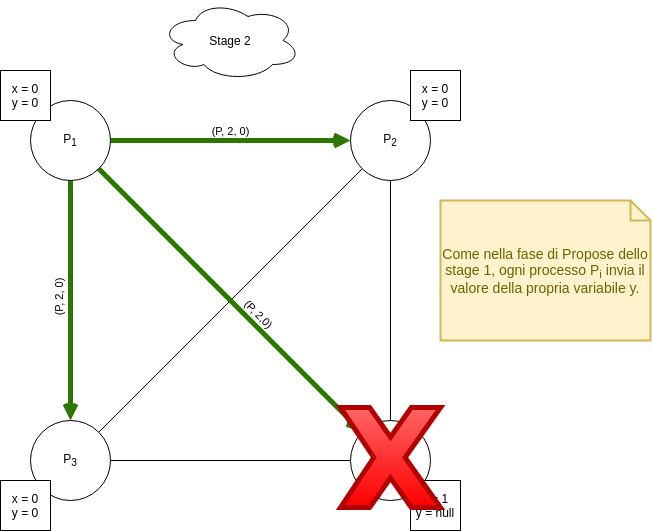
\includegraphics[scale=0.35]{simulazione/simulazione10.png}
\end{figure}
\end{frame}

\begin{frame}{Simulazione - Stage 2 (Propose 2/2)}
\begin{figure}
    \centering
    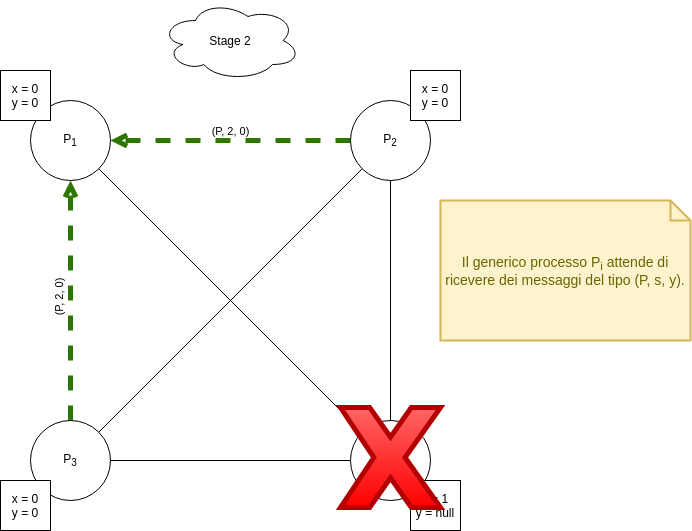
\includegraphics[scale=0.35]{simulazione/simulazione11.png}
\end{figure}
\end{frame}

\begin{frame}{Simulazione - Stage 2 (Decisione)}
\begin{figure}
    \centering
    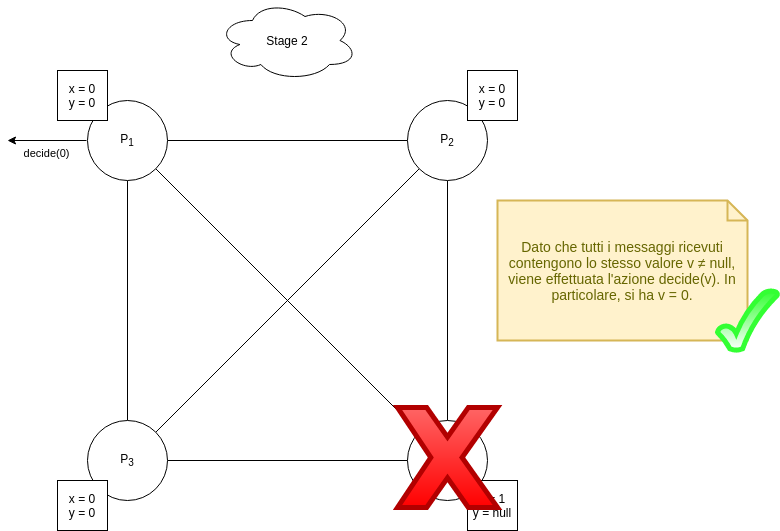
\includegraphics[scale=0.35]{simulazione/simulazione12.png}
\end{figure}
\end{frame}

\subsection{Dimostrazione correttezza}
\begin{frame}{Dimostrazione Correttezza}
    Dimostriamo che l'algoritmo BenOr risolve il problema del consenso.
    
    \begin{block}{Lemma}
        L'algoritmo BenOr garantisce la well-formedness, l'agreement e la validity.
    \end{block}
\end{frame}

\begin{frame}{Dimostrazione Correttezza (Well-formedness) (1/2)} %1
    Va dimostrato che per ogni esecuzione:
    \begin{enumerate}
        \item Non esistono azioni ripetute $init(v)_{i}$, ovvero che ogni processo viene inizializzato al più una volta.
        \item Non esistono azioni ripetute $decide(v)_{i}$, ovvero che ogni processo decide al più una volta.
        \item Ogni $decide(k)_{i}$ è preceduta da una $init(v)_{i}$.
    \end{enumerate}
\end{frame}

\begin{frame}{Dimostrazione Correttezza (Well-formedness) (2/2)} %2
    \textbf{Dimostrazione:}
    \begin{enumerate}
        \item Ogni utente può fare al più una azione di init.
        \item Sebbene i processi continuino la loro esecuzione anche dopo aver deciso un valore, per definizione ogni processo eseguira l'azione di decide una sola volta.
        \item Un processo non inizia la sua esecuzione finchè non riceve un'azione di init. Di conseguenza non può esistere una esecuzione che contenga una decide prima di una init.
    \end{enumerate}
\end{frame}

\begin{frame}{Dimostrazione Correttezza (Validity)}
    Va dimostrato che se ogni processo è inizializzato allo stesso valore \textit{v}, allora \textit{v} è l'unico valore di decisione possibile.
    \newline \newline
    \textbf{Dimostrazione:}
    \begin{enumerate}
        \item<1-> Per ipotesi tutte le azioni $init(v)_{i}$ vengono fatte con lo stesso valore $v$.
        \item<2-> Pertanto nel round di report dello stage 1 tutti i processi invieranno lo stesso messaggio {("R", 1, v)}.
        \item<3-> Segue quindi che tutti i processi riceverann almeno $n - f$ messaggi \mbox{("R", 1, v)}, di consequenza ogni processo invierà un messaggio \mbox{("P", 1, v)}.
        \item<4-> Concludendo tutti i processi riceveranno allora $n - f$ messaggi \mbox{("P", 1, v)} decidendo dunque il valore $v$.
    \end{enumerate}
\end{frame}

\begin{frame}{Dimostrazione Correttezza (Agreement) (1/2)}
    Va dimostrato che tutti i valori di decisione sono uguali.\newline
    \textbf{Dimostrazione:}
    \begin{enumerate}
        \item<1-> Supponiamo che $P_{i}$ decide un certo valore $v$ nello stage $s$, e che sia il primo processo a eseguire una decisione.
        \item<2-> Ciò implica che $P_{i}$ abbia ricetuto $n - f$ mesaggi del tipo \mbox{("P", s, v)}.
        \item<3-> Pertanto ogni altro processo $P_{j}$ che completa lo stage $s$, avrà ricevuto almeno $n - 2f$
        messaggi, questo perchè riceverà gli stessi $n - f$ messaggi che ha ricevuto $P_{i}$, tolti al più $f$ messaggi, nel caso in cui $f$ processi falliscano dopo aver inviato il messaggio a $P_{i}$. Si noti che $n - 2f = (n - f) - f$
    \end{enumerate}
\end{frame}

\begin{frame}{Dimostrazione Correttezza (Agreement) (2/2)}
    \begin{enumerate}
        \setcounter{enumi}{3}
        \item Abbiamo quindi due alternative per ogni altro processo $P_{j}$ che completa lo stage $s$:
        \begin{itemize}
            \item $P_{j}$ ha ricevuto $n - f$ messaggi ("P", s, v) contenenti lo stesso valore $v$.
            \begin{addmargin}[1em]{2em}
            $\implies$ $P_{j}$ decide $v$ e manda a tutti ("R", s, v). 
            \end{addmargin}
            
            \item $P_{j}$ ha ricevuto $n - 2f \leq k < n - f$ messaggi ("P", s, v) contenenti lo stesso valore $v$.
            \begin{addmargin}[1em]{2em}
            $\implies$ $P_{j}$ setta $x := v$ e manda a tutti ("R", s, v). 
            \end{addmargin}
        \end{itemize}
        
        In ogni caso allo stage successivo $s + 1$ tutti i processo riceveranno almeno $n - f$ messaggi ("R", s + 1, v) e invieranno pertanto un messaggio ("P", s + 1, v), di conseguenza tutti i processi riceveranno $n - f$ messagi ("P", s + 1, v) e decideranno quindi v.
    \end{enumerate}
\end{frame}

\begin{frame}{\textit{Quasi certo} VS \textit{Certo}}
    Si noti che probabilità 1 non vuol dire certezza. In seguito dimostreremo che la probabilità di terminazione tende a 1 solo dopo un numero \textbf{infinito} di stage \textit{s}. Quindi possiamo solo essere sicuri che prima o poi accadrà solo se supponiamo di poter aspettare tempi infiniti.
\end{frame}

\begin{frame}{Un esecuzione (finita) senza decisioni}
    Possiamo immaginare un'esecuzione fair del BenOr relativa a $3f+1$ in cui nessuno di questi decide; affinche ciò accada in ogni stage \textit{s} deve accadere che:
    \begin{itemize}
        \item \textit{m} processi, con $f+1 \leq m \leq 2f$, presentano $x = 0$ mentre i rimanenti hanno $x = 1$.
        \item Al termine della fase di Report, tutti i processi avranno $y = null$ %spiegare a voce perchè
        \item Nella fase di Propose assegneranno a \textit{x} un nuovo valore randomico.
        \item \textit{m} processi assegnano $x = 0$ e i rimanenti assegnano $x = 1$
    \end{itemize}
    Nello stage $s + 1$ si ritorna quindi nella situazione iniziale, che potrebbe pertanto ripetersi un numero considerevole di volte.
\end{frame}

\subsection{Dimostrazione terminazione}
\iffalse
\begin{frame}{Confine superiore al tempo di completamento di uno stage}
    MOLTO PROBABILMENTE SI PUO' TOGLIERE A SECONDA DI COME FORMULI LA TERMINAZIONE.
    OVVERO SE LA SI PONE IN TERMINI DI TEMPO E' NECESSARIA, SE LA SI PONE IN TERMINI DI STAGE ALLORA LA SI PU0' TOGLIERE
    Possiamo innanzituto dimostrare che:
    \begin{block}{Lemma}
        In ogni esecuzione fair dell'algoritmo BenOr in cui un'evento di \textit{init} occorre su tutte le porte, ogni processo non guasto completa un numero infinito di stage.\newline
        Inoltre, sia \textit{l} un confine superiore al tempo di completamento di ogni task dei processi, e \textit{d} un confine superiore al tempo di consegna di ogni messaggio; allora ogni processo non guasto completa ogni stage entro un tempo $O(s(d+l))$, calcolato a partire dall'ultimo evento di \textit{init}.
    \end{block}
\end{frame}
\fi

\begin{frame}{Probabilità di terminazione}
    \begin{block}{Lemma}
        Per ogni stage \textit{s}, tutti i processi decideranno entro lo stage successivo $s+1$ con una probabilità \textit{p} tale che:
        \begin{center}
        \huge
            $p \geq 1 - (1-\frac{1}{2^n})^s$
        \end{center}
    \end{block}
\end{frame}

\begin{frame}{Dimostrazione (1/8)}
    Se $s = 0$ allora la dimostrazione è banale infatti si ha che:
    \vspace{0.3cm}
    \begin{center}
        \Large
        $1 - (1 - \frac{1}{2^n})^s = 1 - (1 - \frac{1}{2^n})^0 = 1 - 1 = 0$
    \end{center}
    \normalsize
    \vspace{0.3cm}
    I.e., si sta dicendo che ogni processo termina con probabilità $p \geq 0$, il che è ovvio.
\end{frame}

\begin{frame}{Dimostrazione (2/8)}
    Consideriamo ora il caso $s \geq 1$. \newline
    Dimostriamo innanzitutto che alla fine dello stage s, ogni processo imposta \textit{x} allo stesso valore \textit{v} con una probabilità $p \geq \frac{1}{2^n}$. 
    \begin{enumerate}
        \item<1-> Sia $\alpha$ l'esecuzione più corta per cui un processo $P_{i}$ ha ricevuto $n - f$ messaggi ("R", s, *).
        \item<2-> Se almeno $f + 1$ di questi messaggi contengono lo stesso valore \textit{v}, allora diciamo che \textit{v} è un valore \textit{buono} per $\alpha$. 
        \item<3-> Sono possibili due casi:
        \begin{itemize}%!!!!! DA RIELABORARE QUESTO PUNTO
            \item E' presente un solo valore \textit{buono}, i.e., $P_{i}$ ha ricevuto o almeno $f + 1$ \mbox{("R", s, 0)} oppure almeno $f + 1$ ("R", s, 1).
            \item Sono presenti due valori \textit{buoni}, i.e., $P_{i}$ ha ricevuto almeno $f + 1$ \mbox{("R", s, 0)} e almeno $f + 1$ ("R", s, 1).
        \end{itemize}
    \end{enumerate}
\end{frame}

\begin{frame}{Dimostrazione (3/8): Un solo valore buono}
    \begin{enumerate}
        \setcounter{enumi}{3}
        \item<1-> Nel caso in cui \underline{$P_{i}$ ha ricevuto un solo valore \textit{buono} \textit{v}}, ogni altro processo $P_{j}$ avrà ricevuto almeno 1 ($f + 1 - f = 1$) messaggi del tipo ("R", s, v).
        \item<2-> Non appena $P_{j}$ avrà ricevuto $n - f$ messaggi ("R", s, *), non potrà inviare un messagio del tipo ("P", s, $\overline{v}$), in quanto per definizione può farlo solamente se ha rivecuto esattamente $n - f$ copie di $\overline{v}$, ma per quanto detto soprà sappiamo che ciò è impossibile in quanto tra gli $n - f$ messaggi che ha ricevuto contengono almeno 1 copia di $v$.
        \item<3-> Pertanto ogni messaggio ("P", s, *) che verrà inviato conterrà o il valore \textit{v} oppure \textit{null}.
    \end{enumerate}
\end{frame}

\begin{frame}{Dimostrazione (4/8): Un solo valore buono}
    \begin{enumerate}
        \setcounter{enumi}{6}
        \item<1-> Nel momento in cui un processo $P_{j}$ riceve $n - f$ messaggi ("P", s, v) allora, o avrà ricevuto almeno $n - 2f$ messaggi contenenti il valore \textit{buono} $v$ e imposterà $x$ a $v$, oppure ne avrà ricevuti di meno e sceglierà il valore di $x$ in manierò random.
        \item<2-> La probabilità che tutti i processi che scelgono in maniera random, scelgano lo stesso valore $v$ è: $\geq (\frac{1}{2})^n$, in quanto ogni processo ha probabilita $\frac{1}{2}$ di scegliere il valore $v$.  
    \end{enumerate}
\end{frame}

\begin{frame}{Dimostrazione (5/8): Due valori buoni}
    \begin{enumerate}
        \setcounter{enumi}{8}
        \item<1-> Nel caso in cui \underline{$P_{i}$ ha ricevuto due valori \textit{buoni}}, ogni altro processo $P_{j}$ avrà ricevuto almeno 1 messaggio del tipo ("R", s, 0) e almeno 1 messaggio del tipo ("R", s, 0).
        \item<2-> Non appena $P_{j}$ avrà ricevuto $n - f$ messaggi ("R", s, *), non potrà inviare un nè messagi del tipo ("P", s, 0), nè messagi del tipo ("P", s, 1).
        \item<3-> Pertanto ogni messaggio ("P", s, *) che verrà inviato conterrà o il valore \textit{null}.
    \end{enumerate}
\end{frame}

\begin{frame}{Dimostrazione (6/8)}
    \begin{enumerate}
        \setcounter{enumi}{11}
        \item<1-> Ogni processo riceverà quindi unicamente messaggi del tipo ("P", s, \textit{null}), dovendo quindi impostare il valore di \textit{x} in maniera random.
        \item<2-> Anche in questo caso la probabilità che tutti i processi impostino \textit{x} allo stesso valore è: $\geq (\frac{1}{2})^n$.
    \end{enumerate}
\end{frame}

\begin{frame}{Dimostrazione (7/8)}
    \begin{enumerate}
        \setcounter{enumi}{13}
        \item Abbiamo quindi dimostrato che in entrambi i casi alla fine dello stage \textit{s}, con probabilità $p \geq \frac{1}{2^n}$, ogni processo imposta \textit{x} allo stesso valore \textit{v}.
        \item Per \textbf{negazione} si ha che la probabilità \textit{p} che \textbf{non} venga scelto un valore unico per \textit{x} è $p \leq 1 - \frac{1}{2^n}$.
        \item Poichè la le scelte che vengono fatte in uno stage sono \textbf{indipendenti} tra di loro abbiamo che, la probabilità \textit{p} che non venga scelto un valore unico per \textit{x} nei primi \textit{s} stage è: $p \leq (1 - \frac{1}{2^n})^s$
        \item Ancora una volta per \textbf{negazione} si ha che la probabilità \textit{p} che venga scelto un valore unico per \textit{x} entro lo stage \textit{s} è: $p \geq 1 - (1 - \frac{1}{2^n})^s$ 
    \end{enumerate}
\end{frame}

\begin{frame}{Dimostrazione (8/8)}
    \begin{enumerate}
        \setcounter{enumi}{17}
        \item Se tutti i processi impostano lo stesso valore per \textit{x} alla fine di uno stage \textit{s}, allora per definizione dell'algoritmo tutti i processi \textit{decideranno} quel valore di \textit{x} alla fine dello stage $s + 1$.
        \item Per quanto detto prima la probabilità \textit{p} che venga scelto un valore uni per \textit{x} entro lo stage \textit{s} è: $p \geq 1 - (1 - \frac{1}{2^n})^s$. 
        \item Dunque la probabilità di decidere un valore entro lo stage $s + 1$ è:
        \begin{center}
            \Large
            $p \geq 1 - (1 - \frac{1}{2^n})^s$.
        \end{center}
    \end{enumerate}
\end{frame}

\begin{frame}{Terminazione con probabilità 1}
    E' facile vedere che:
    \begin{center}
        \Large
        $\lim_{s\to\infty} 1 - (1 - \frac{1}{2^n})^s = 1$
    \end{center}
    Questo vuol dire che al crescere del numero di stage la probabilità di decidere un valore entro lo stage $s+1$. \newline \newline
    All'infinito questo valore diventa pari a 1. Ovvero si ha che con probabilità 1, prima o poi tutti i processi decidono.
\end{frame}

{
    \beamertemplatenavigationsymbolsempty
    \setbeamertemplate{footline}{}
    \usebackgroundtemplate{
        \adjustbox{trim=-8cm 0 0 -4.5cm}{
            \transparent{0.3}\includesvg[scale=0.4,keepaspectratio=true]{unito-logo.svg}
        }
    }
    \begin{frame}{Ringraziamenti}
    \begin{textblock*}{\textwidth}(5mm, 32mm)
        \Huge Grazie per l'attenzione!
    \end{textblock*}
    \begin{textblock*}{0.6\textwidth}(5mm, 75mm)
        \begin{block}{Riferimenti bibliografici:}
            \tiny Nancy A. Lynch, \textit{Distributed Algorithms}, 1996 \\
            Marcos Kawazoe Aguilera e Sam Toueg, \textit{Correctness Proof of Ben-Or’s Randomized Consensus Algorithm}, 1998
        \end{block}
    \end{textblock*}
    \end{frame}
    \addtocounter{framenumber}{-1}
}

\end{document}